\documentclass[a4paper,
fontsize=11pt,
%headings=small,
oneside,
numbers=noperiodatend,
parskip=half-,
bibliography=totoc,
final
]{scrartcl}

\usepackage[babel]{csquotes}
\usepackage{synttree}
\usepackage{graphicx}
\setkeys{Gin}{width=.4\textwidth} %default pics size

\graphicspath{{./plots/}}
\usepackage[ngerman]{babel}
\usepackage[T1]{fontenc}
%\usepackage{amsmath}
\usepackage[utf8x]{inputenc}
\usepackage [hyphens]{url}
\usepackage{booktabs} 
\usepackage[left=2.4cm,right=2.4cm,top=2.3cm,bottom=2cm,includeheadfoot]{geometry}
\usepackage{eurosym}
\usepackage{multirow}
\usepackage[ngerman]{varioref}
\setcapindent{1em}
\renewcommand{\labelitemi}{--}
\usepackage{paralist}
\usepackage{pdfpages}
\usepackage{lscape}
\usepackage{float}
\usepackage{acronym}
\usepackage{eurosym}
\usepackage{longtable,lscape}
\usepackage{mathpazo}
\usepackage[normalem]{ulem} %emphasize weiterhin kursiv
\usepackage[flushmargin,ragged]{footmisc} % left align footnote
\usepackage{ccicons} 
\setcapindent{0pt} % no indentation in captions

%%%% fancy LIBREAS URL color 
\usepackage{xcolor}
\definecolor{libreas}{RGB}{112,0,0}

\usepackage{listings}

\urlstyle{same}  % don't use monospace font for urls

\usepackage[fleqn]{amsmath}

%adjust fontsize for part

\usepackage{sectsty}
\partfont{\large}

%Das BibTeX-Zeichen mit \BibTeX setzen:
\def\symbol#1{\char #1\relax}
\def\bsl{{\tt\symbol{'134}}}
\def\BibTeX{{\rm B\kern-.05em{\sc i\kern-.025em b}\kern-.08em
    T\kern-.1667em\lower.7ex\hbox{E}\kern-.125emX}}

\usepackage{fancyhdr}
\fancyhf{}
\pagestyle{fancyplain}
\fancyhead[R]{\thepage}

% make sure bookmarks are created eventough sections are not numbered!
% uncommend if sections are numbered (bookmarks created by default)
\makeatletter
\renewcommand\@seccntformat[1]{}
\makeatother

% typo setup
\clubpenalty = 10000
\widowpenalty = 10000
\displaywidowpenalty = 10000

\usepackage{hyperxmp}
\usepackage[colorlinks, linkcolor=black,citecolor=black, urlcolor=libreas,
breaklinks= true,bookmarks=true,bookmarksopen=true]{hyperref}
\usepackage{breakurl}

%meta
%meta

\fancyhead[L]{C. Winkler\\ %author
LIBREAS. Library Ideas, 39 (2021). % journal, issue, volume.
\href{http://nbn-resolving.de/}
{}} % urn 
% recommended use
%\href{http://nbn-resolving.de/}{\color{black}{urn:nbn:de...}}
\fancyhead[R]{\thepage} %page number
\fancyfoot[L] {\ccLogo \ccAttribution\ \href{https://creativecommons.org/licenses/by/4.0/}{\color{black}Creative Commons BY 4.0}}  %licence
\fancyfoot[R] {ISSN: 1860-7950}

\title{\LARGE{Digitalisierung am Deutschen Museum – alles andere als retro}}% title
\author{Christian Winkler} % author

\setcounter{page}{1}

\hypersetup{%
      pdftitle={Digitalisierung am Deutschen Museum – alles andere als retro},
      pdfauthor={Christian Winkler},
      pdfcopyright={CC BY 4.0 International},
      pdfsubject={LIBREAS. Library Ideas, 39 (2021).},
      pdfkeywords={Digitalisierung, Deutsches Museum, Bibliotheksgeschichte},
      pdflicenseurl={https://creativecommons.org/licenses/by/4.0/},
      pdfcontacturl={http://libreas.eu},
      baseurl={http://libreas.eu},
      pdflang={de},
      pdfmetalang={de}
     }



\date{}
\begin{document}

\maketitle
\thispagestyle{fancyplain} 

%abstracts
\begin{abstract}
\noindent
\textbf{Kurzfassung}: Die Digitalisierung und Onlinepräsentation von
Buchbeständen ist in der Welt der Bibliotheken schon lange kein Novum
mehr. Der Artikel beschreibt am Beispiel der Projekte der Bibliothek des
Deutschen Museums die verschiedenen Formen von Bestandsdigitalisierung
in chronologischer Reihenfolge. Dabei wird nicht nur die Genese eines
konkreten Digitalisierungskonzeptes verständlich, sondern auch generell
Kriterien bibliothekarischer Digitalisierung und ihrer Vorzüge
nachvollziehbar.

\begin{center}\rule{0.5\linewidth}{0.5pt}\end{center}

\noindent\textbf{Abstract}: The digitization and online presentation of book
collections has long since ceased to be a novelty in the world of
libraries. Using the projects of the library of the Deutsches Museum as
an example, the article describes the various forms of collection
digitization in chronological order. In doing so, not only the genesis
of a concrete digitization concept becomes clear, but also general
criteria of library digitization and its advantages.
\end{abstract}

%body

\hypertarget{digitalisierung-im-bibliothekarischen-kontext}{%
\section{Digitalisierung im bibliothekarischen
Kontext}\label{digitalisierung-im-bibliothekarischen-kontext}}

Digitalisierung gehört zum Alltagsgeschäft von Bibliotheken und das seit
über zwanzig Jahren. Ein Artikel über Digitalisierung an einer (relativ)
kleinen Bibliothek kann sicherlich in der Fachwelt nicht aufgrund
innovativer Revolutionen punkten -- vor allem nicht in der
Retrospektive. Sehr wohl aber kann das Interesse dafür geweckt werden,
wie denn der Beitrag einer Museumsbibliothek zu einer digitalisierten
Welt bisher ausgesehen hat, welche Probleme aufgetreten sind und wie
diese angegangen werden konnten. Dies ist zumindest die Hoffnung des
Verfassers dieses übergreifenden Werkstattberichts. So werden spezielle
Probleme am Beispiel deutlich, aber auch generell wird ersichtlich,
inwiefern der \enquote{gute alte Zettelkatalog}, Produkt
bibliothekarischer Arbeit und Metadatenfundgrube, digital gewandelt --
Stichwort: Metadatenmanagement -- nicht überflüssig geworden ist. Am
Beispiel der Bibliothek des Deutschen Museums wird in dieser Hinsicht
deutlich, dass die Bibliothek sich durch Digitalisierung nicht selbst
abschafft, sondern durch Fortführung dieser bibliothekarischen
Grundaufgaben Mehrwerte schafft. Im Verbund mit den anderen Säulen des
Museums -- Ausstellungen und Archiv -- leistet sie ihren Beitrag zu
einer gemeinsamen digitalen Strategie,\footnote{\url{https://digital.deutsches-museum.de/about/digital-strategy/}
  Zugriff am 08.02.2021.} deren Ursprung bereits seit den Gründungstagen
angelegt ist, aber digital weit über die Museumsinsel Münchens
hinausgeht.

\begin{figure}
\centering
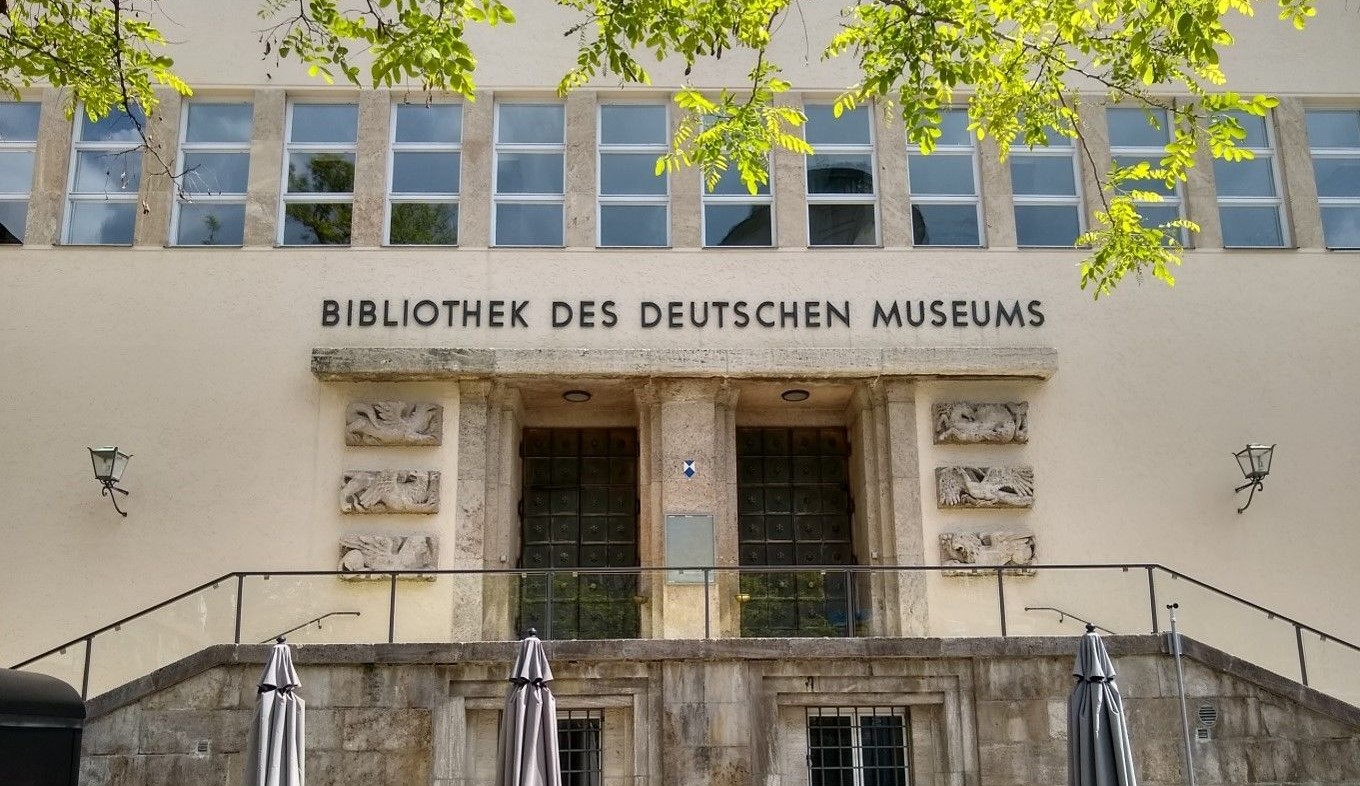
\includegraphics[width=.9\textwidth]{img/Abb1.jpg}
\caption{Als geographischer Ort: Spezial- und Fachbibliothek für technik-
und wissenschaftshistorisch Interessierte}
\end{figure}

\hypertarget{die-grundvoraussetzung-digitale-erfassung-der-metadaten-der-bestuxe4nde-im-katalog-und-deren-einspielung-in-den-verbund}{%
\section{Die Grundvoraussetzung: Digitale Erfassung der Metadaten
der Bestände im Katalog und deren Einspielung in den
Verbund}\label{die-grundvoraussetzung-digitale-erfassung-der-metadaten-der-bestuxe4nde-im-katalog-und-deren-einspielung-in-den-verbund}}

Bibliotheken haben seit jeher die Aufgabe, Bücher und generell Medien zu
sammeln und verfügbar zu machen.\footnote{Ewert, Gisela {[}u.a.{]}:
  Bibliotheken. Die Definition der Bibliothek. In: Bibliotheksdienst 33
  (1999) 6, S. 957--971.} Im Falle der Spezial- und Forschungsbibliothek
des Deutschen Museums bedeutet dies bereits seit der Gründung einen
Sammel- und Erschließungsauftrag für Naturwissenschaft, Technik und
deren Geschichte.\footnote{Hilz, Helmut (2017): Die Bibliothek des
  Deutschen Museums. Geschichte -- Sammlung -- Bücherschätze. München:
  Deutsches Museum, S. 72.} Um diese Erschließung zu ermöglichen, werden
Kataloge geführt, die in gewisser Weise die Inhaltsverzeichnisse der
Bibliotheken sind. Diese haben im Verlauf der Bibliotheksgeschichte
unterschiedliche Formen gehabt: Bandkataloge, Zettelkataloge\ldots{} In
jedem Fall sind sie durch die enthaltenen Metadaten wie die Findbücher
in den Archiven der Schlüssel zur effizienten Nutzung. Auch digital
nutzt es wenig, zu wissen, dass \enquote{alles im Netz} ist, wenn das
Finden der gewünschten Information mit ermüdender und langfristiger
Bildschirmarbeit verbunden ist.

Seit 1995/96 katalogisiert die Bibliothek des Deutschen Museums in den
Verbundkatalog des Bibliotheksverbunds Bayern (BVB). Um rückwirkend
sinnvoll den gesamten Bestand verzeichnet zu haben und damit die
analogen Metadatenverzeichnisse digital nutzbar zu machen, schloss sich
eine Zeit der Retrokatalogisierung an. Dieses Vorhaben war für eine
Museumsbibliothek mit relativ großem Bestand nicht trivial. Inzwischen
bewegt sich der Bestand auf die Millionengrenze zu und ein nicht zu
unterschätzender Teil des Bestandes ist gemäß dem speziellen
Sammlungsauftrag deutschlandweit selten vorhanden, sodass
Fremddatenübernahme nicht flächendeckend möglich war.

Zusätzlich zu den Katalogkästen waren die seit der Gründerzeit geführten
Sachkataloge, welche Aufsätze, Zeitungsartikel und graue Literatur nach
Themen verzeichnen, ins Digitale zu überführen. Hier wurde ein
hausinternes Projekt durchgeführt, um die große Menge an Katalogkarten
einzuscannen und zumindest als Imagekatalog verfügbar zu machen. Mit der
Verbundkatalogisierung wurde zudem die Weiterführung des analogen
Instruments obsolet.

Das Vorhalten qualitativ guter Metadaten in bestenfalls übergreifenden
Systemen bildet die unabdingbare Voraussetzung für digitale Projekte und
dies in zweierlei Hinsicht: Zum einen verlangt der Anschluss an Verbünde
immer eine strenge Beachtung (und gegebenenfalls externe Kontrolle) der
eigenen Erschließungspraxis, zum anderen ist die digitale
Langzeitarchivierung beim Verbund besser gewährleistet. Schließlich
wurde der Vorteil für den Nutzenden rasch ersichtlich: Zum Jahresende
1999 ging der Onlinekatalog ins Netz.

\begin{figure}
\centering
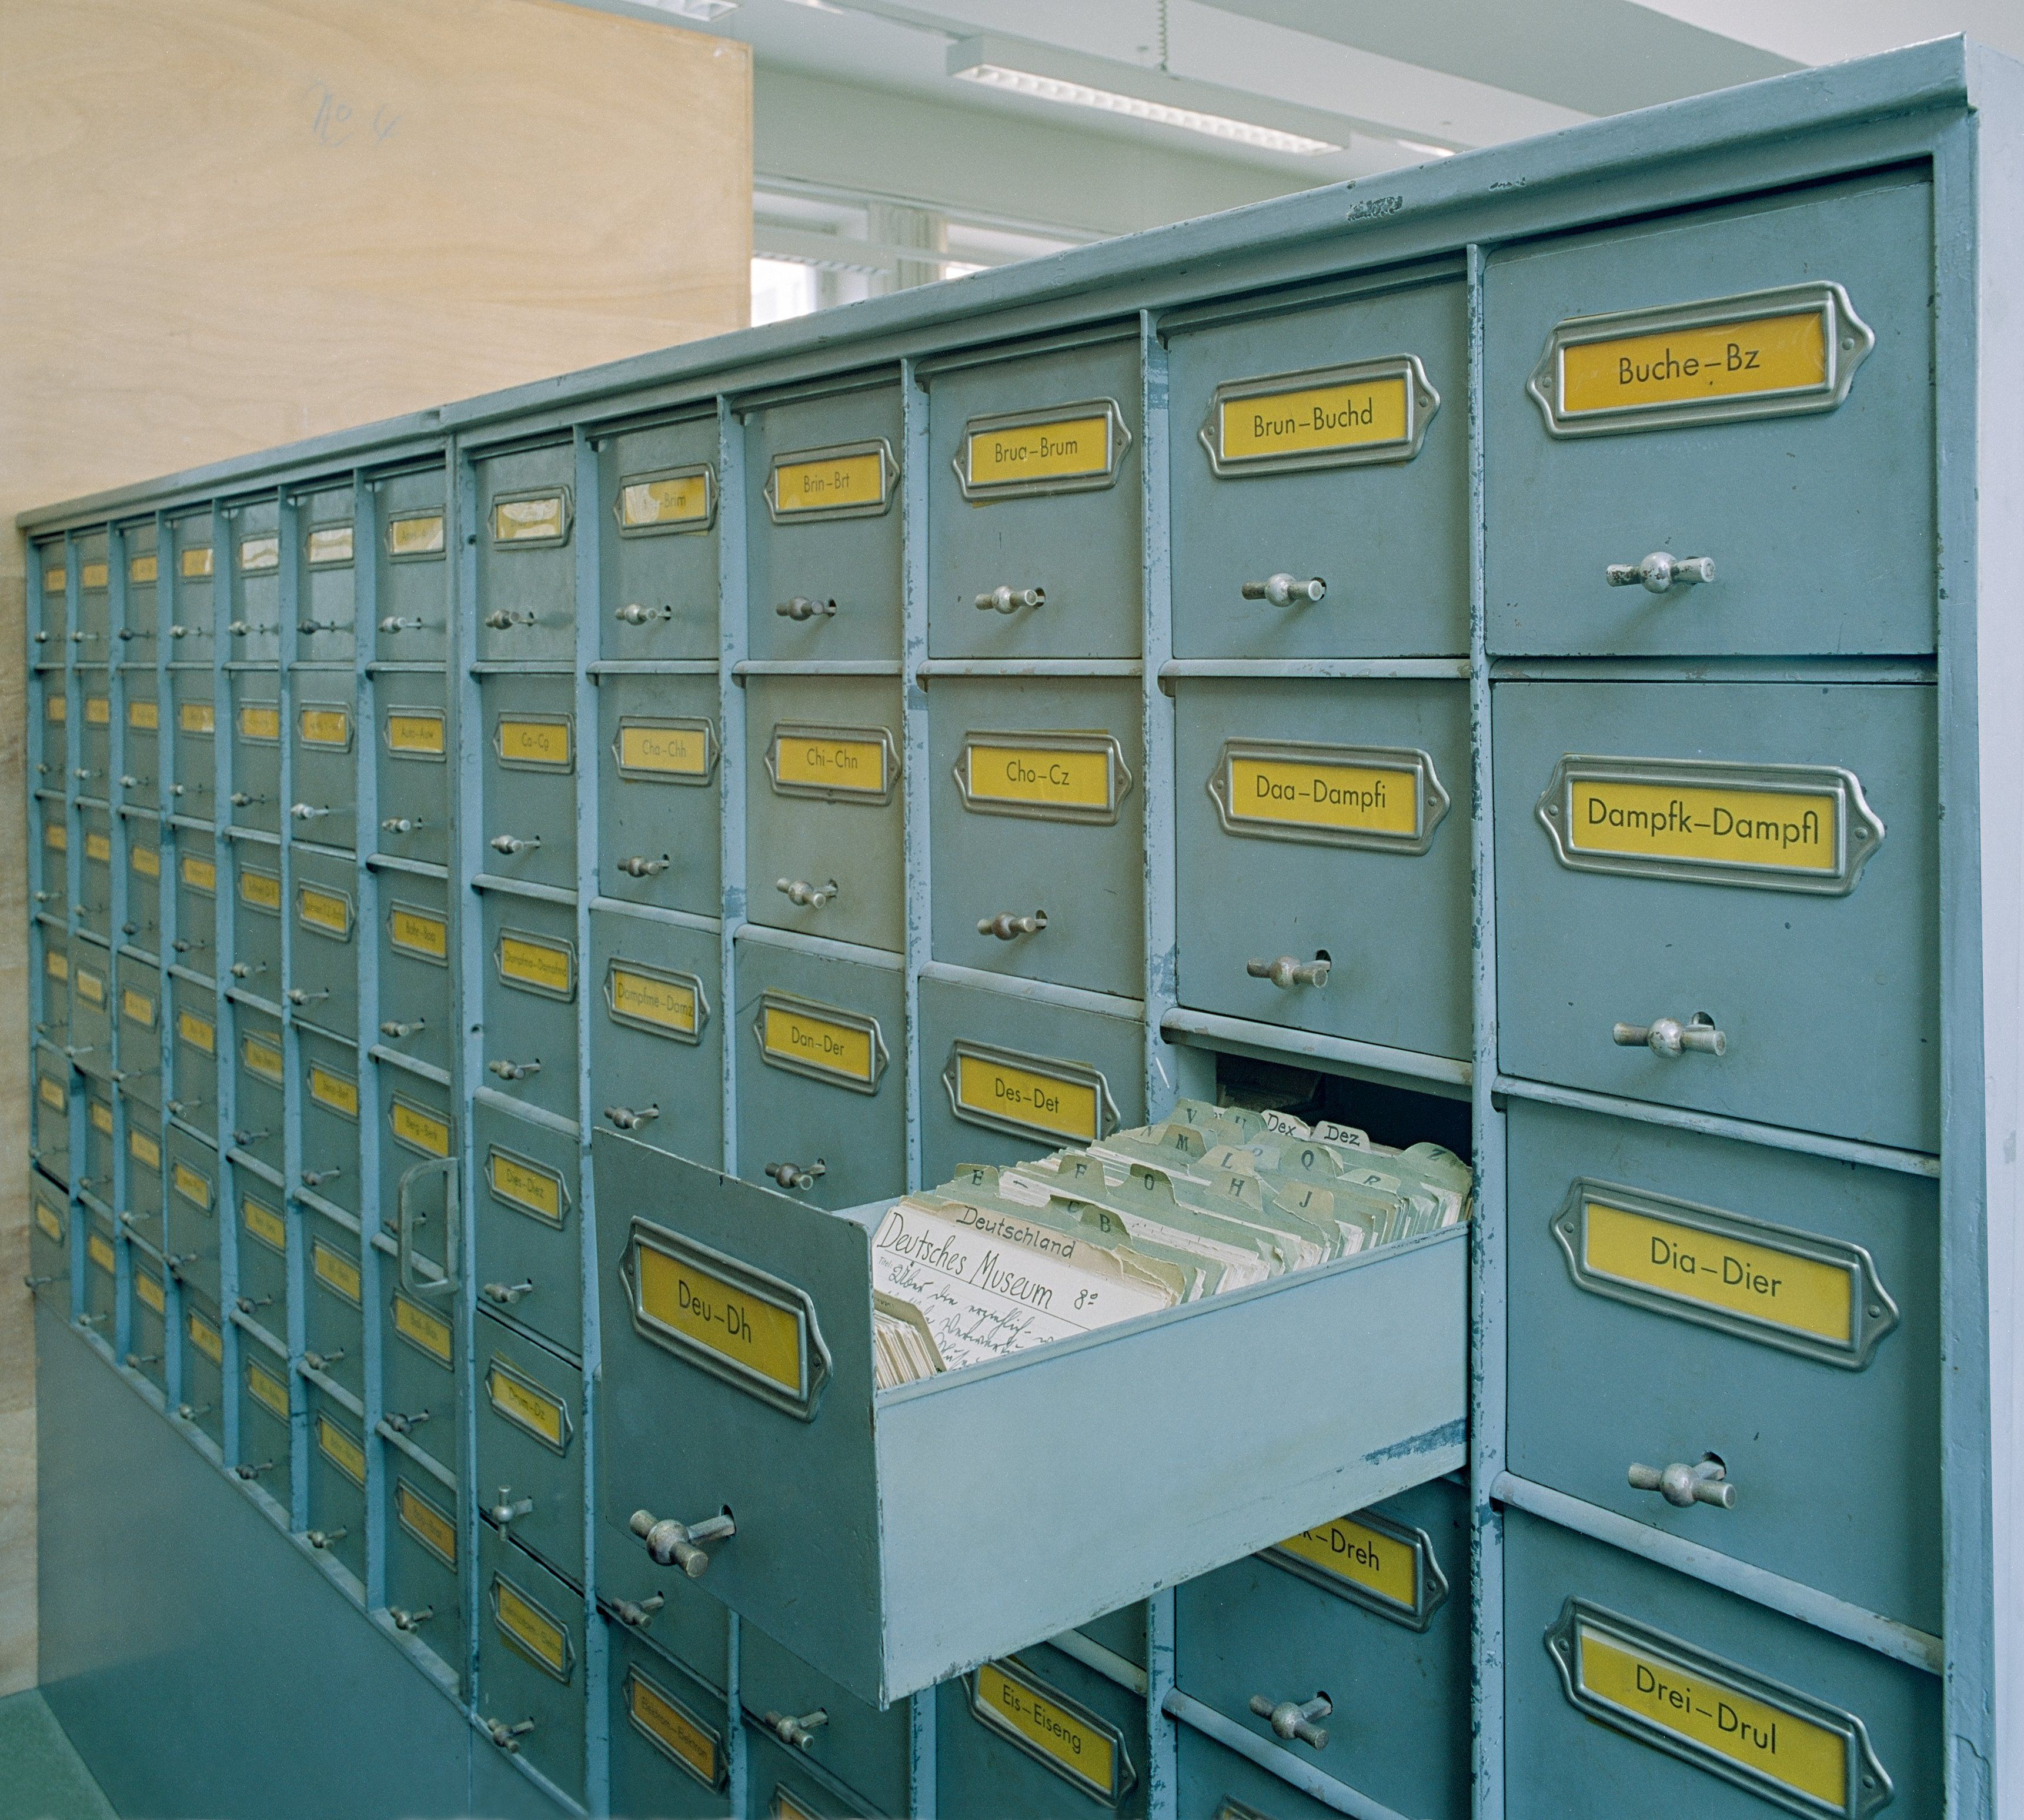
\includegraphics[width=.70\textwidth]{img/Abb2.jpg}
\caption{Der Erste Schritt der Digitalisierung: Umwandlung des
Zettelkatalogs oder modern: der Metadaten}
\end{figure}

\hypertarget{erste-vorsichtige-schritte}{%
\section{Erste (vorsichtige)
Schritte}\label{erste-vorsichtige-schritte}}

Ist diese (Daten-)Ebene essentiell wichtiger Bestandteil eines
Digitalisats,\footnote{Altenhöner, Reinhard {[}u.a.{]}: Digitalisierung
  von Kulturgut. In: Rolf Griebel {[}u.a.{]} (Hg.): Praxishandbuch
  Bibliotheksmanagement. Berlin: De Gruyter, 2015, S. 763--811, hier S.
  793--801.} so kann man bei ihr noch nicht von einer vollumfänglichen
Digitalisierung des Bestandes sprechen. Hierbei erwarten Nutzende nicht
mehr nur Angaben zu Titeln, sondern auch die Möglichkeit, Zugriff auf
den Scan der Werke zu haben. Seit 2004 verfügt die Bibliothek des
Deutschen Museums mit dem ersten Buchscanner über das notwendige
Werkzeug. Ohne festgesteckte Projektziele diente dieses allerdings
zunächst der Reaktion auf Digitalisierungswünsche einzelner KuratorInnen
des Museums und die in dieser Art produzierten Scans waren kein direkter
Gewinn für die Nutzenden der Bibliothek oder die virtuelle
Öffentlichkeit. Nach dem Motto \enquote{Learning by Doing} wurden die
technischen Notwendigkeiten umgesetzt: Ein Laufwerk für die zu
erwartenden Digitalisate wurde eingerichtet, eine Ablagestruktur und ein
Benennungssystem für die Dateien entwickelt.

\begin{figure}
\centering
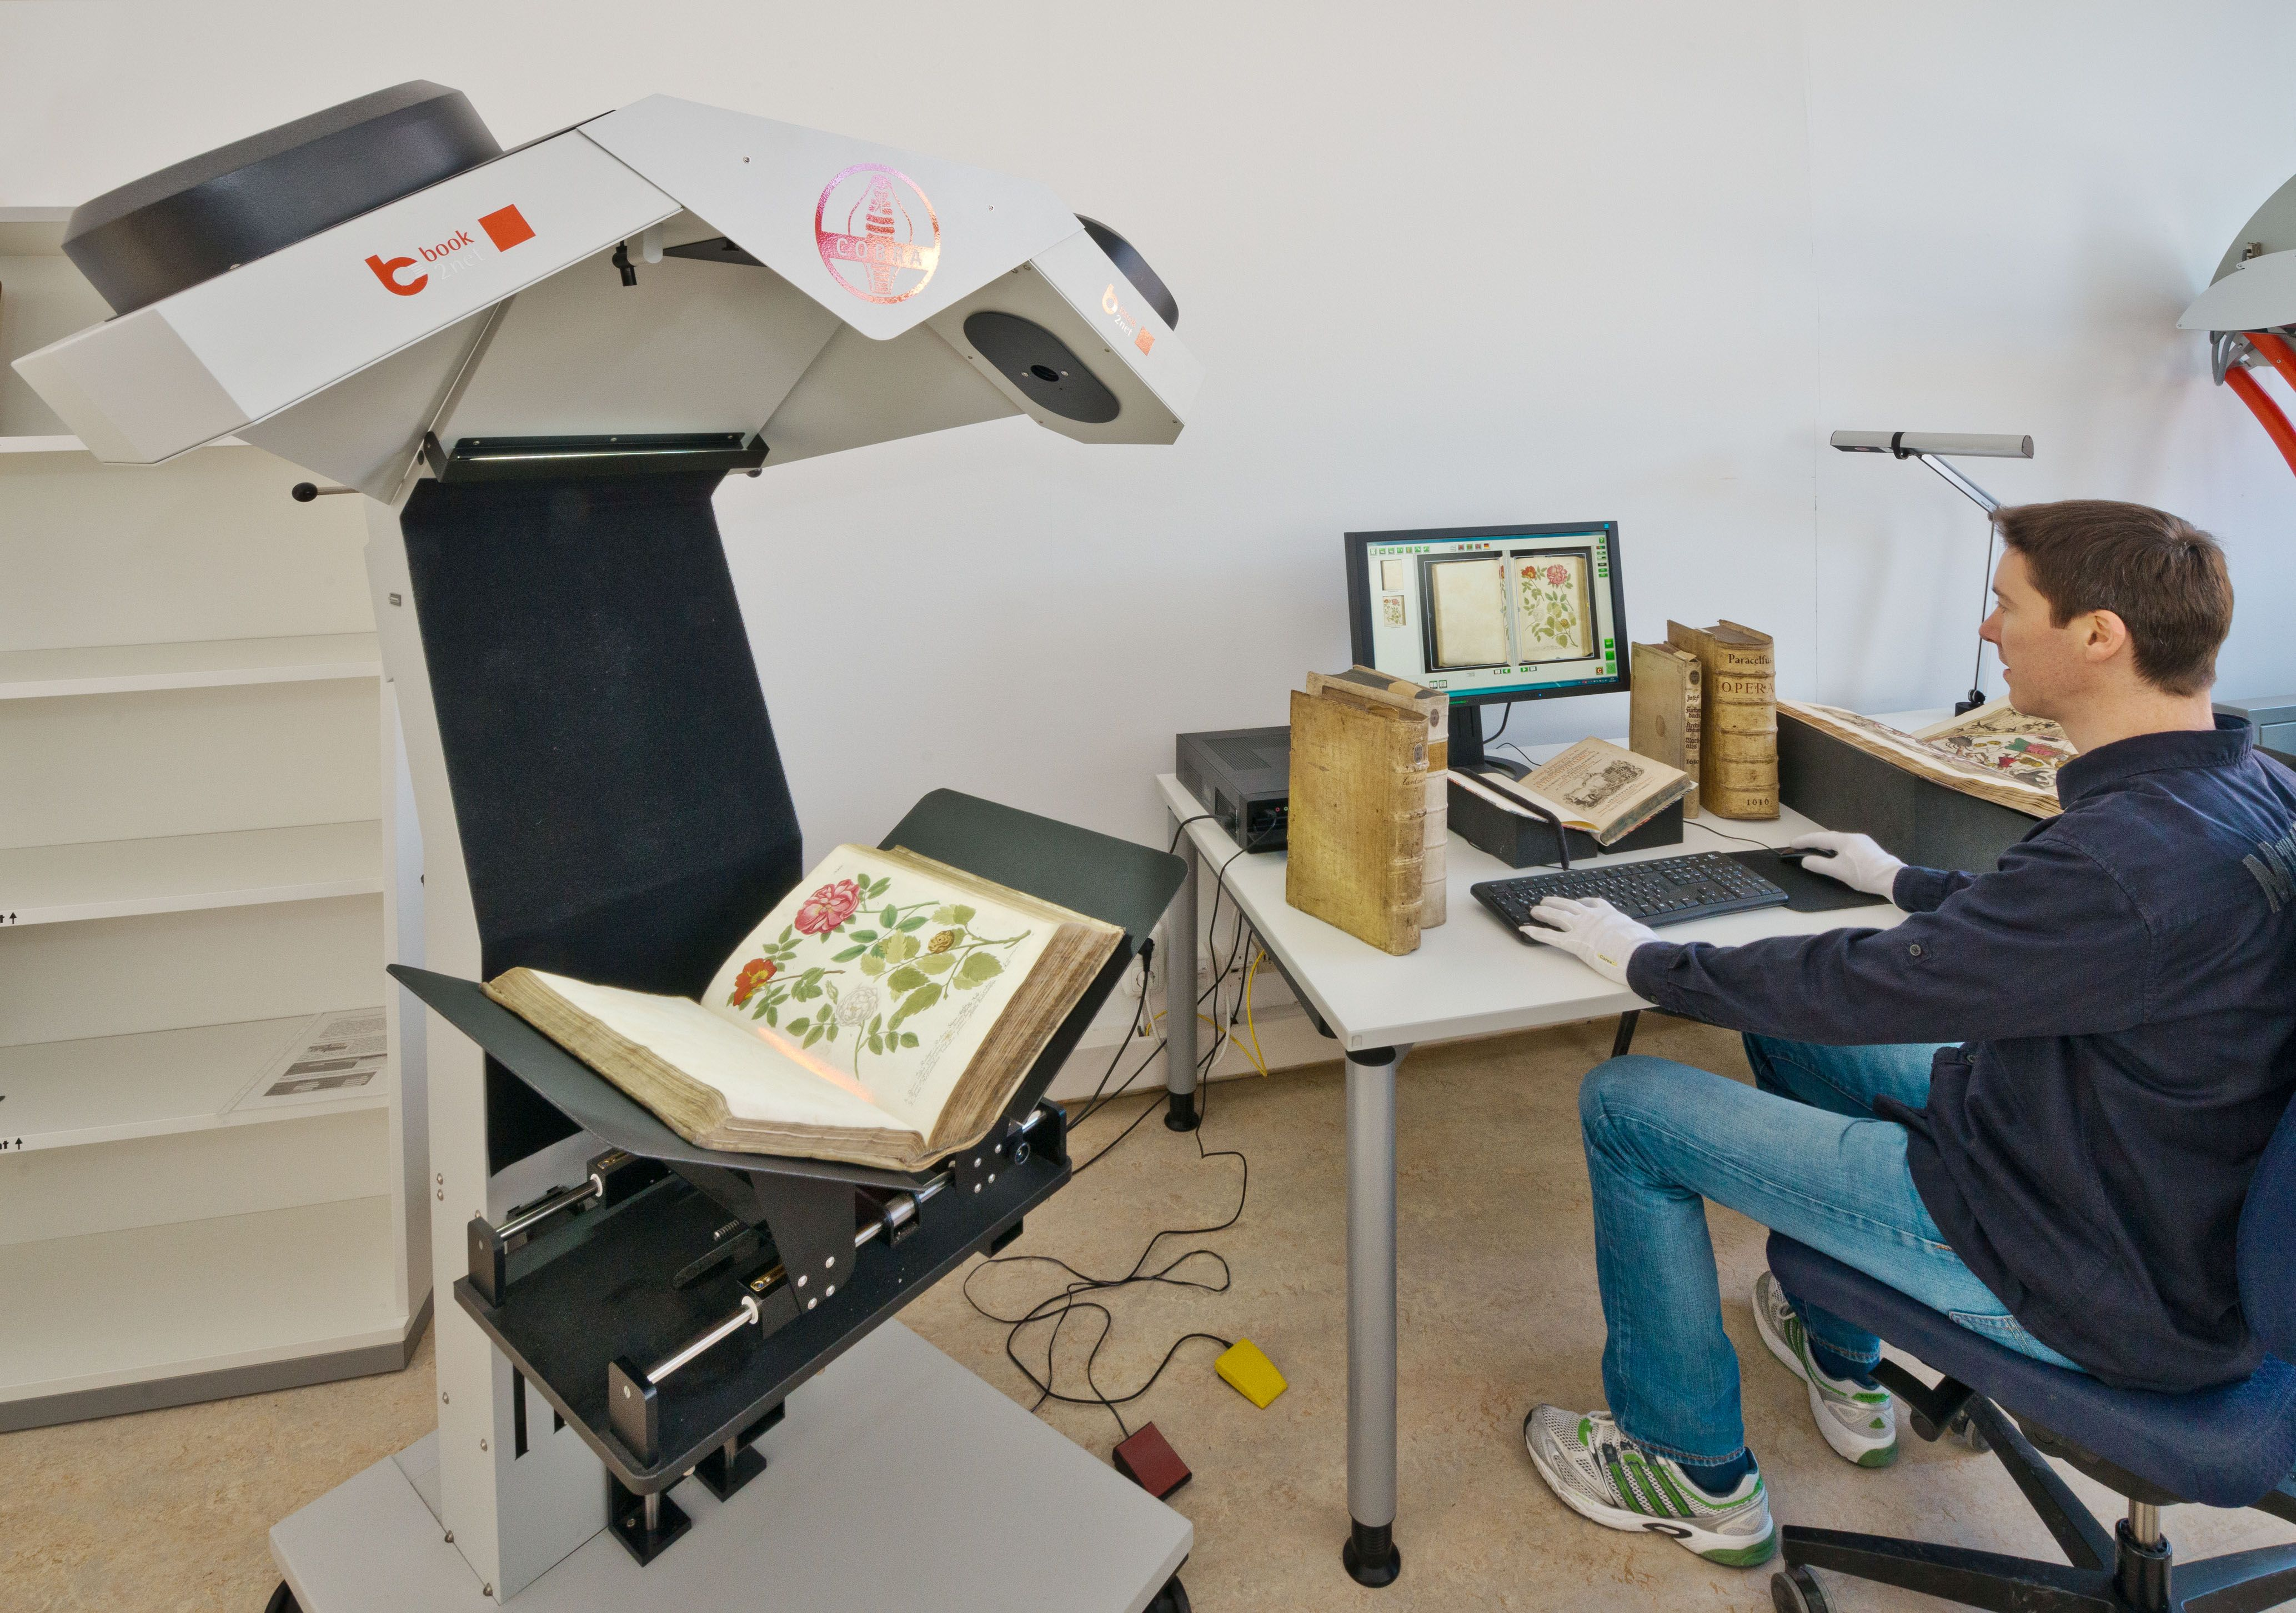
\includegraphics[width=.70\textwidth]{img/Abb3.jpg}
\caption{Boutique-Digitalisierung erfordert Manpower und Sorgfalt}
\end{figure}

Mag diese Dienstleistung für die Forschenden vor Ort eine nette
Ergänzung zu früheren Kopieraufträgen sein, wird insbesondere im
deutschlandweiten Kontakt mit WissenschaftlerInnen der Nutzen einer
dezentralen Bereithaltung von Literatur deutlich: Zwar ist die
Bibliothek in gewisser Weise die Hausbibliothek der anwesenden
Forschenden und einschlägig interessierter MünchnerInnen, dem
Verständnis nach ist der Sammelauftrag bundesweit für das erwähnte
Fachprofil zu verstehen. Entsprechend sind die für das Museum
angeschafften Werke zwar Präsenzbestand, stehen aber der Forschung per
Fernleihe zur Verfügung. Abgesehen von der postalischen Lösung ist die
digitale Bereitstellung älterer Literatur eine naheliegende Alternative,
um den geografisch in Deutschland verteilten Forschenden kleiner
Disziplinen unnötige Reisen nach München zu ersparen.

Um die Notwendigkeit einer Bestellung oder gar einer Forschungsreise
bewerten zu können, kamen nun weitere (digitale) Erschließungsmethoden
zum Einsatz: Erste merkliche Verbesserung brachte auch für die Nutzenden
der Bibliothek des Deutschen Museums der Einstieg des Verbunds in die
Kataloganreicherung, welche der Bibliotheksverbund Bayern 2006 einführte
und hierfür sowohl Bearbeitungswerkzeug und Anleitungen bereitstellte.
Die an die Katalogeinträge angehängten gescannten Inhaltsverzeichnisse
haben insbesondere bei nichtssagenden Titeln oder Sammelbänden einen
eindeutigen Wert für jeden, der sich im Katalog fragt, ob das
entsprechende Werk bestellenswert ist. Als Spezialbibliothek mit Werken,
die ansonsten eher selten in Deutschland zu finden sind, entschied man
sich schnell, diese Anreicherung für die hochspezielle Erwerbung
anzuwenden. Das Einscannen von Inhaltsverzeichnissen ist bis heute neben
der verbalen Sacherschließung (Verschlagwortung) eine nicht zu
vernachlässigende Daueraufgabe der Bibliothek geblieben.

\hypertarget{erstes-projekt-astronomie-rara-in-kooperation-mit-der-eth-zuxfcrich-2010}{%
\section{Erstes Projekt: Astronomie-Rara in Kooperation mit der
ETH Zürich
2010}\label{erstes-projekt-astronomie-rara-in-kooperation-mit-der-eth-zuxfcrich-2010}}

Schließlich war in mehreren Etappen die Zeit reif für das Herzstück der
Digitalisierung, die digitale Reproduktion von analog vorliegenden
Werken. Durch eine glückliche Fügung erfolgte dies zunächst durch die
Beteiligung an einem Projekt: Anlässlich des Jahres der Astronomie 2009
ergab sich eine Kooperation mit der ETH Zürich. Auf einem gemeinsamen
Portal\footnote{\url{https://astronomie-rara.ethbib.ethz.ch/} Zugriff am
  08.02.2021.} stellten die beiden Bibliotheken 191 bedeutsame Werke der
Astronomiegeschichte der Öffentlichkeit zur Verfügung. Die
Zusammenarbeit mit einer großen Bibliothek brachte es mit sich, dass die
Bibliothek Einblicke in die Anforderungen an derartige Projekte und vor
allem auch der entsprechenden Abläufe erlangte. Fürs Erste begnügte man
sich in Zürich damit, die großformatigen Scans im TIFF-Format per
Festplatte zugeschickt zu bekommen, folgende Arbeitsschritte wurden samt
und sonders in der Schweiz erledigt.

In Ermangelung zufriedenstellender erschwinglicher Softwarelösungen für
den Scan-Workflow setzte die Bibliothek auf Eigenentwicklung, die sich
vor allem für das Haus, aber auch in Projekten wie der Digitalisierung
umweltgeschichtlicher Werke in Zusammenarbeit mit dem Rachel Carson
Center for Environment and Society\footnote{\url{https://www.carsoncenter.uni-muenchen.de/index.html}
  Zugriff am 08.02.2021.} verdient machte. Diese Eigenentwicklung
bündelte notwendige Arbeitsschritte anderer digitaler Werkzeuge,
koordinierte Prozesse wie die Umwandlung der TIFF-Dateien in
Präsentationsformate sowie die Verknüpfung mit den Metadaten des
Katalogs und ermöglichte zudem eine Anreicherung des Katalogisats um
Schlagwörter und Strukturdaten -- Arbeitsschritte, bei denen andere
Workflowentwicklungen noch keine befriedigenden Lösungen anboten.

\href{img/Abb4.jpg}{Auch digital sehenswert: Die Buchschätze des
Astronomie-Rara-Projekts mit der ETH Zürich}

\hypertarget{vd18-20142016}{%
\section{VD18 2014--2016}\label{vd18-20142016}}

Waren mit dem Astronomie-Projekt die ersten Schritte quasi als
Juniorpartner der ETH Zürich gegangen, trat das Deutsche Museum als
Player der retrospektiven deutschen Nationalbibliographie\footnote{Fieseler,
  Christian: Das Verzeichnis Deutscher Drucke des 18. Jahrhunderts (VD
  18): Ziele, Entwicklung und aktueller Stand). -- In BuB 68 (2016) 7,
  S. 402--405.} für das 18. Jahrhundert in Erscheinung.
Grundvoraussetzung war auch hier, dass in seiner Sammlung teilweise
unikaler Bestand an Spezialliteratur bereits seit den Gründungstagen
gesammelt wurde. Um den Schritt des Scannens bei geringem Öffnungsgrad
wertvoller alter Bücher und die Möglichkeit, schnell(er) umzublättern,
zu geben, wurde ein zusätzlicher (Cobra-)Scanner angeschafft.

Die Ansprüche an die Digitalisate sind bereits durch den
förderpolitischen Motor, die Deutsche Forschungsgemeinschaft
(DFG),\footnote{DFG (2013): DFG-Praxisregeln \enquote{Digitalisierung}.
  Online verfügbar unter
  \url{http://www.dfg.de/formulare/12/_151/12/_151/_de.pdf}, Zugriff am
  08.02.2021.} festgelegt. Ansprüche an Metadaten mussten besonders
erfüllt werden, die Verknüpfung von Scan und Metadaten, im besten Fall
noch angereichert um Strukturdaten, musste vom Haus selbst erledigt
werden. Mit 300 zu digitalisierenden Werken des Altbestands auch vom
Umfang her eine Steigerung. Um diesen Ansprüchen Herr zu werden, wurde
erneut auf softwaretechnische Eigenentwicklung gesetzt.

\begin{figure}
\centering
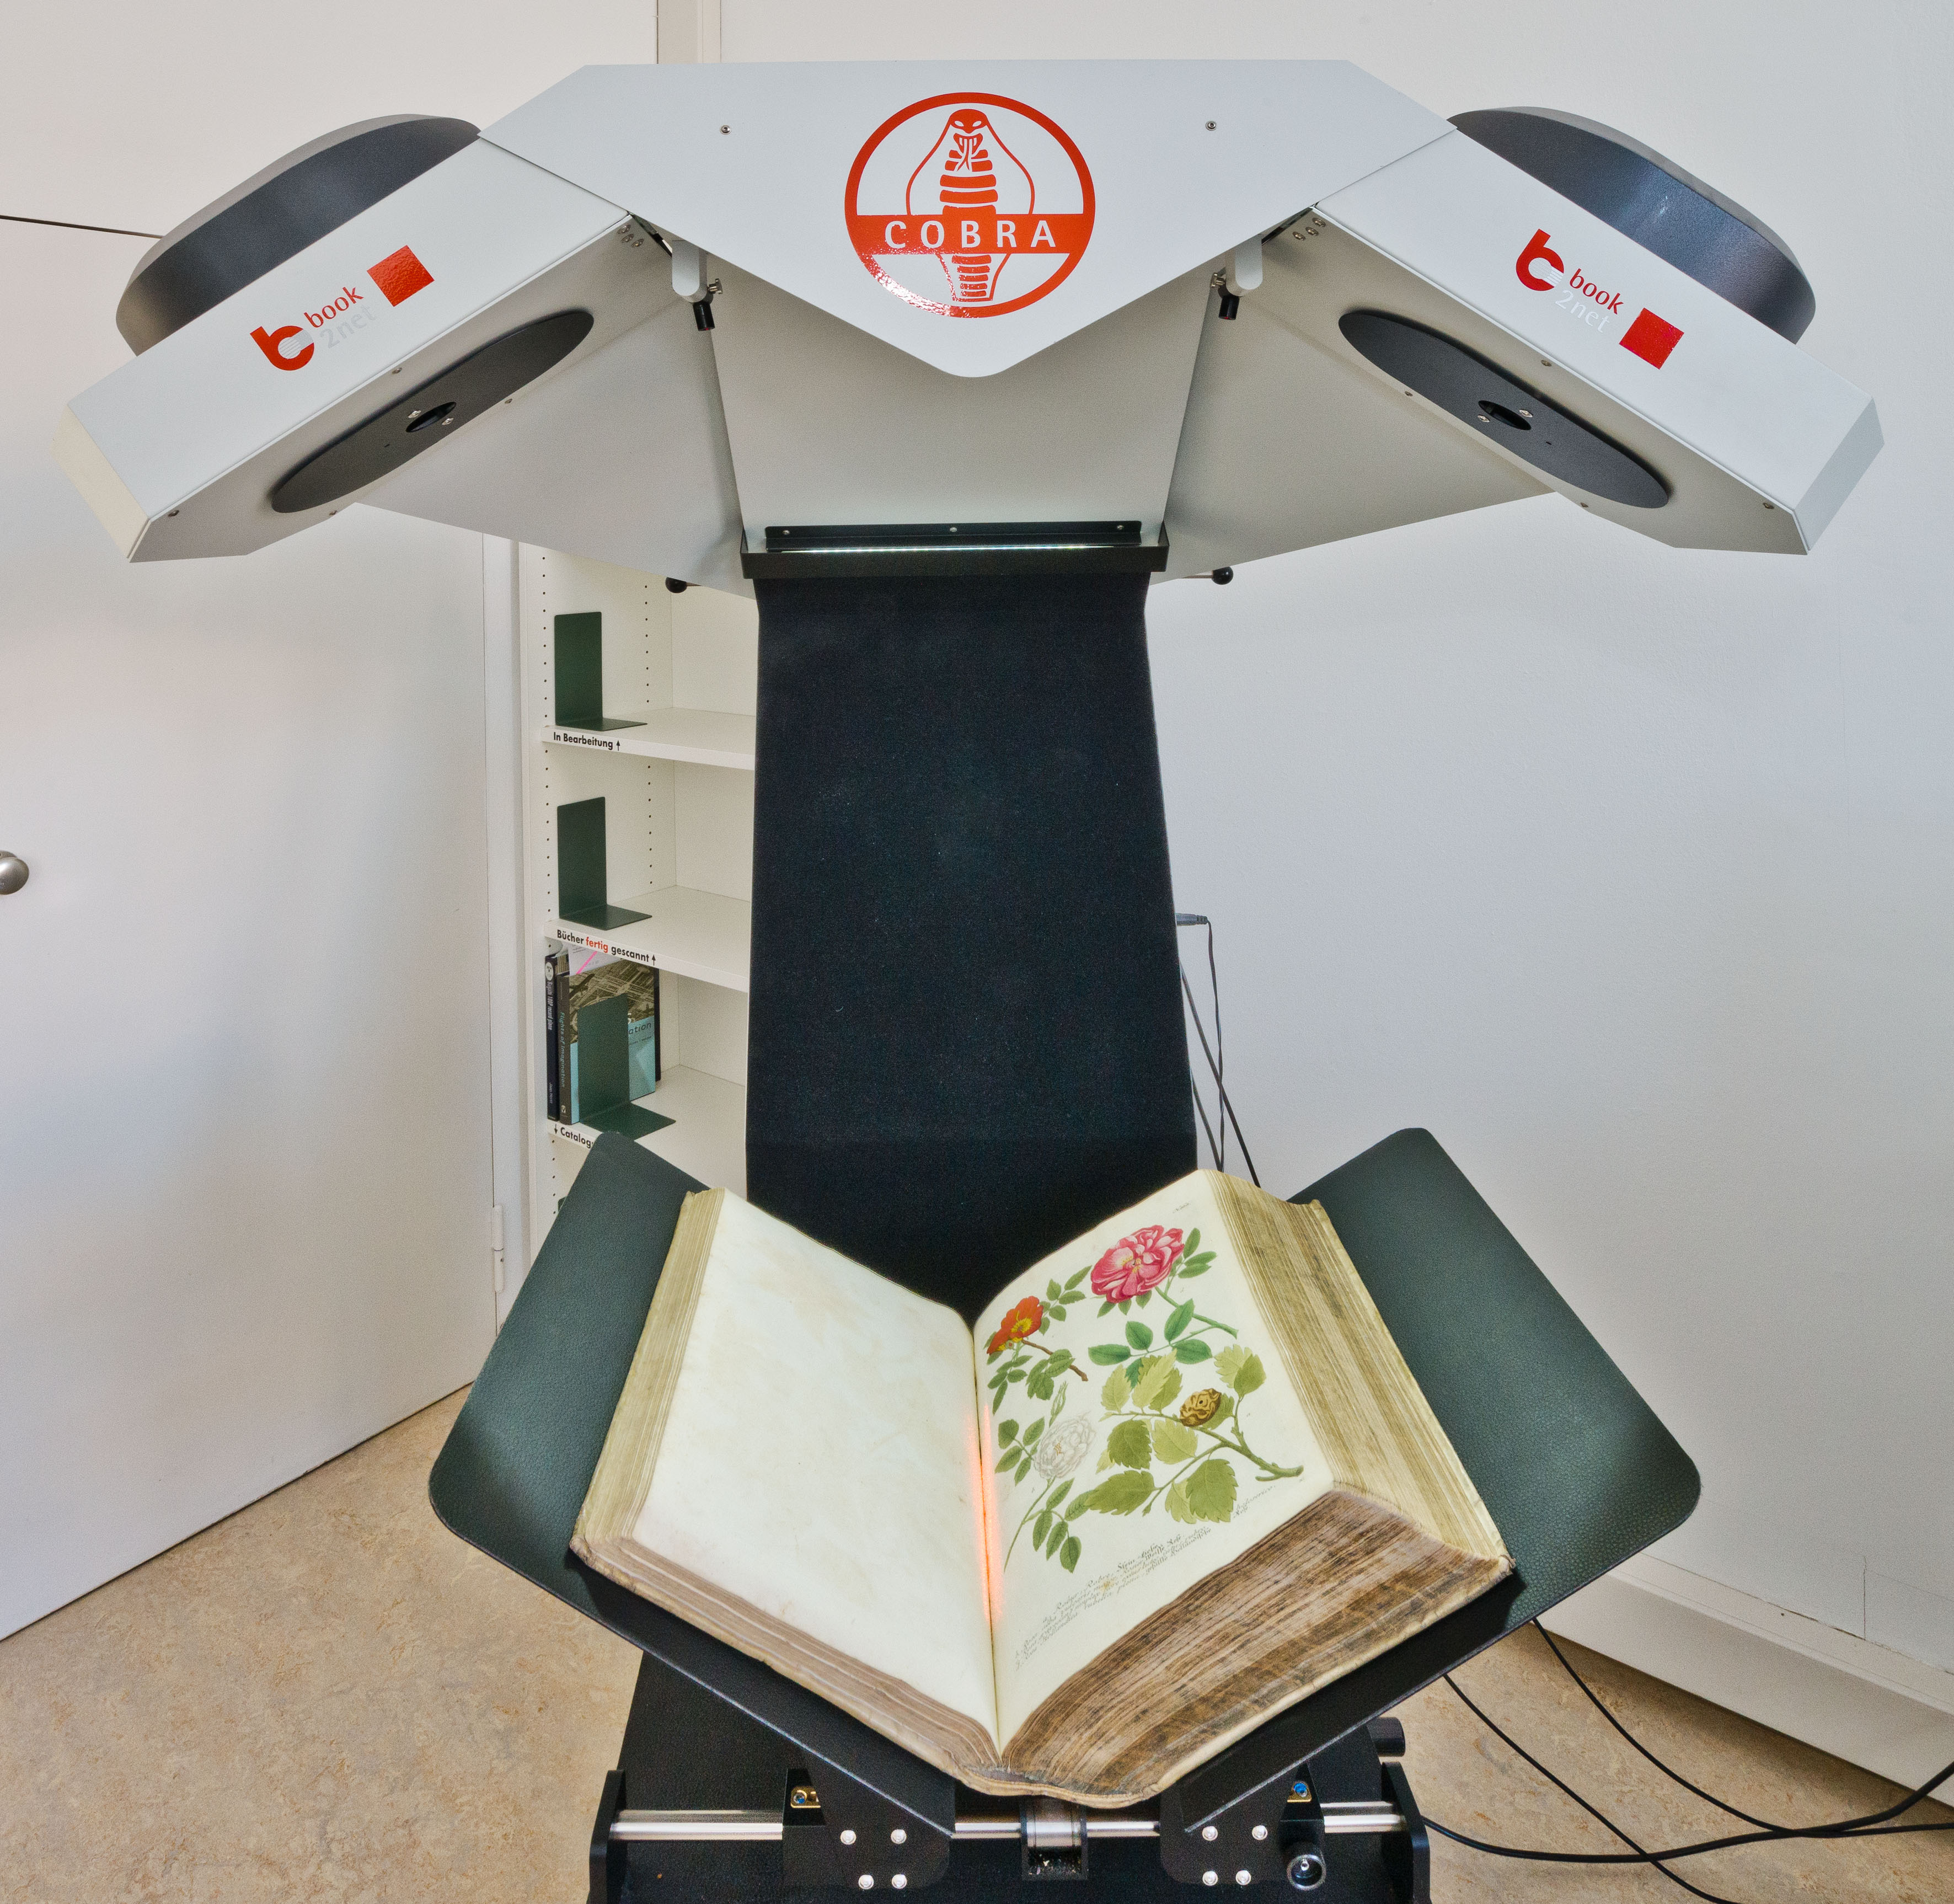
\includegraphics[width=.70\textwidth]{img/Abb5.jpg}
\caption{Die Technik, unverzichtbarer, aber nicht einziger Bestandteil
guter Digitalisierung}
\end{figure}

\hypertarget{einstieg-in-die-massendigitalisierung-die-kooperation-mit-google-books}{%
\section{Einstieg in die Massendigitalisierung: Die Kooperation
mit Google
Books}\label{einstieg-in-die-massendigitalisierung-die-kooperation-mit-google-books}}

Im Anschluss an die erfolgreichen Verhandlungen der Bayerischen
Staatsbibliothek (BSB) mit Google und der für beide Seiten erfolgreichen
Durchführung des Projekts in den Jahren nach 2008\footnote{Hilpert,
  Wilhelm: 10 Jahre Partnerschaft mit Google. Auswirkungen und Spuren an
  der Bayerischen Staatsbibliothek. -- In: Klaus Ceynowa {[}u.a.{]}
  (Hg.): Bibliotheken: Innovation aus Tradition: Rolf Griebel zum 65.
  Geburtstag. -- Berlin/Boston: De Gruyter, 2015, S. 258--266.} stieg
auch die deutsche Bibliothekslandschaft ins Massengeschäft ein. Nach den
positiven Erfahrungen der BSB entstand im Deutschen Museum die Idee,
diese Möglichkeit ebenfalls zu nutzen.

Zwar führt der Wunsch einer Bibliothek, die Bestände zu digitalisieren,
nicht zwangsläufig zu einer Kooperation, denn Google kann rein
ökonomisch nicht daran interessiert sein, ein Kooperationsprojekt für
eine Bibliothek aufzusetzen, deren Bestände grosso modo bereits bei
großen Bibliotheken \enquote{abgegriffen} wurden und entsprechend bei
Google Books zu finden sind. Im Fall des Deutschen Museums waren eher
inhaltliche Gründe vorrangig:

\begin{itemize}
\item
  Die Bibliothek des Deutschen Museums verfügt über einen bedeutenden
   Altbestand (libri rari) von 16.000 Werken aus dem
  Bereich der  Geschichte der Technik und der
  Naturwissenschaften.
\item
  Als quasi Hausbibliothek für Technikhistoriker verfügt die
   Bibliothek über eine umfangreiche Sammlung in der
   Technikgeschichte, die zum Bereich der \enquote{kleinen
  Fächer}\footnote{\url{https://www.kleinefaecher.de/} Zugriff am
    08.02.2021}  zählt. Ist die Bereitschaft, ein
  derartiges \enquote{kleines Fach}  literaturtechnisch
  aus dem Bibliotheksetat umfassend zu bedienen,  bei den
  meisten Universitätsbibliotheken gering, so hat das 
  Deutsche Museum hier zusätzlich in gewisser Weise einen Auftrag
   als Archivbibliothek.
\item
  Zusätzlich zur im Buchhandel erschienenen Literatur wird
   einschlägige graue Literatur gesammelt.
\item
  Patentschriften und Adressbücher: Handelt es sich bei diesen zwei
   Gattungen sicherlich nicht um sehr verbreiteten
   Bibliotheksbestand, sind sie durch den
  technikhistorischen  \linebreak Schwerpunkt des Hauses für die
  einschlägige Forschung von großem  Nutzen.
  Glücklicherweise sind sie nicht aufgrund von Säureschaden
   des schlechten Papiers entsorgt worden, wie es
  andernorts gerade  bei den Adressbüchern und
  Branchenverzeichnissen häufig der Fall  war: Das
  Veralten der enthaltenen Information ist häufig ebenso 
  Grund zur Aussonderung, im Fall des Deutschen Museums jedoch ist
   dies allerdings eher ein Grund für die Aufbewahrung: Um
   Erkenntnisse etwa über Industrialisierungsprozesse zu
  gewinnen,  sind Branchenverzeichnisse eine ergiebige
  Quelle. Schließlich  gehörte und gehört zur
  technikhistorischen Forschung auch oft eine  Recherche
  bezüglich Entwicklungen und ihrer Vermarktung.
\end{itemize}

2016 schließlich kam der Startschuss für die Kooperation des Museums mit
Google und damit auch die Digitalisierung mit Google Books. Die Gründe
auf der Museumsseite für eine derartige Kooperation sind leicht
ersichtlich, denn eine Digitalisierung von 50.000 gemeinfreien Bänden
war und ist bei der vorhandenen Personaldecke nicht zu stemmen. Im
Vergleich zur Boutique-Digitalisierung\footnote{Ceynowa, Klaus:
  Massendigitalisierung für die Wissenschaft -- Zur
  Digitalisierungsstrategie der Bayerischen Staatsbibliothek. In: Rolf
  Griebel {[}u.a.{]} (Hg.): Information, Innovation, Inspiration. 450
  Jahre Bayerische Staatsbibliothek. München: Saur, 2008, S. 241--252,
  hier S. 245.}, wie sie oben beschrieben wurde, war die
Public-Private-Partnership mit dem amerikanischen Digitalgiganten von
ganz anderen Überlegungen geprägt und hatte für ein kleines Haus ganz
andere Herausforderungen zu bieten.

Ist bei der Digitalisierung mit Google ein sehr personalintensiver und
zeitaufwändiger Faktor, das eigentliche Scannen, quasi ausgelagert, so
bleiben der Bibliothek wichtige Aufgaben. Einerseits sind diese
bibliothekarisch, denn mit Hilfe des Katalogs wurden die Werke
identifiziert, die urheberrechtlich unbedenklich sind und diese zu
Lieferungen zusammengefasst. Dabei kam es insbesondere beim Bestand der
libri rari, der kostbaren Altbestandssammlung, zu zahlreichen
Umarbeitungen und Aktualisierungen der Katalogeinträge. In Bezug auf
Zeitschriften mussten Jahrgangsbände systematisch in den Katalog
aufgenommen werden, damit diese verbuchbar, sprich: ausleihbar, waren.
Andererseits ist der Abtransport in das Digitalisierungszentrum von
Google durchaus auch eine logistische Herausforderung und so sorgte der
Ruf: \enquote{Google ist da!} für hektische Betriebsamkeit in Bibliothek
und Magazin.

\begin{figure}
\centering
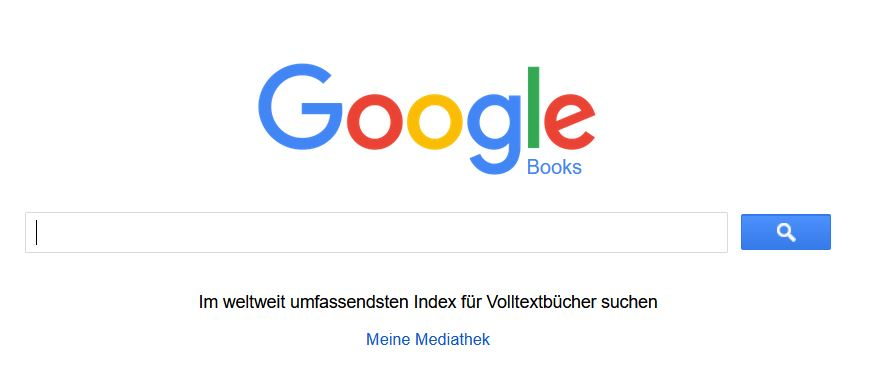
\includegraphics[width=.70\textwidth]{img/Abb6.jpg}
\caption{Sicherlich hohe Sichtbarkeit garantiert die Einspielung der
digitalen Bestände des Google Projekts bei Google Books. Zusätzlich
werden die Werke auch im Deutschen Museum Digital verfügbar sein.}
\end{figure}

Sicherlich können Digitalisate, die bei Google Books angezeigt werden,
in vielerlei Hinsicht nicht mit den Produkten der Hausdigitalisierung
mithalten. Nicht ausgeklappte Falttafeln, zerschnittene Titelblätter,
mitgescannte Finger, das sind Phänomene, für die sich erst im Vollzug
eine gewisse Sensibilität entwickelt hat und für welche Lösungen
gefunden werden müssen. Ebenfalls irrig ist die Annahme, dass
Massendigitalisierung die Kunst der (digitalen) Editorik übernehmen
könnte. Trotzdem, für eine Bereitstellung großer Textmengen ist die
Massendigitalisierung ein inzwischen auch am Deutschen Museum bewährtes
Verfahren und nach Abschluss der Hauptphase im Jahr 2019 kommt es auch
in Zukunft zu Lieferungen an Google, denn mit den fortschreitenden
Jahren verschiebt sich ebenfalls die Grenze der urheberrechtlichen
Unbedenklichkeit. Abgesehen von der Tatsache, dass ohne Google nicht mit
dieser Menge an Digitalisaten zu rechnen gewesen wäre, so ist die bei
Google durchgeführte automatische Texterkennung (Optical Character
Recognition, OCR) in Fachkreisen anerkannt und sorgt für einen Zugewinn
an Metadaten der eingescannten Titel: Die weitgehende Durchsuchbarkeit
des Textes. Insbesondere bei den erwähnten Branchenverzeichnissen und
Patentschriften wird so ein wahrer \enquote{digitaler Mehrwert}
geschaffen und das konservatorische Problem entschärft.

\hypertarget{beteiligung-am-fachinformationsdienst-fid-geschichtswissenschaft-seit-2016}{%
\section{Beteiligung am Fachinformationsdienst (FID)
Geschichtswissenschaft (seit
2016)}\label{beteiligung-am-fachinformationsdienst-fid-geschichtswissenschaft-seit-2016}}

Ihrer Rolle als Partnerin \enquote{in der digitalen Welt} wurde die
Bibliothek des Deutschen Museums noch auf anderer Ebene gerecht:
Zusammen mit der Bayerischen Staatsbibliothek übernahm sie im FID
Geschichtswissenschaft die Betreuung der Subdisziplin
Technikgeschichte,\footnote{Bunge, Eva {[}u.a.{]}: Neue Services für die
  Technikgeschichte: Fachinformationsdienst Geschichtswissenschaft
  (FID). -- In: Technikgeschichte 85 (2018), S. 195--201.} seit Beginn
der zweiten Förderphase zusätzlich die Fächer Umwelt- und
Naturwissenschaftsgeschichte. Da das DFG-Programm generell der digitalen
Priorität verpflichtet ist, leistet auch die Bibliothek des Deutschen
Museums ihren Teil an der Digitalisierung vergriffener Werke. Mit dem
Beirat für Wissenschafts-, Technik- und Umweltgeschichte hat man sich
auf das Thema der frühen Atomforschung verständigen können. Diese
Digitalisierung hat Monographien zum Gegenstand. Hierfür verwendet die
Bibliothek weiterhin den erprobten Workflow, der als Eigenproduktion nun
an seine Grenzen stößt. Eine Anpassung an Standards insbesondere im
Bereich der Zeitschriftendigitalisierung ist nicht zuletzt aufgrund der
verwendeten Programmiersprache nicht ohne weiteres möglich.
Glücklicherweise entspricht die derzeitige Situation in Deutschland
nicht mehr denen der Pionierzeit, als die Zeichen auf Eigenentwicklung
standen: So liegt mit \emph{Kitodo. Key to digital objects} ein
Workflowmanagementsystem vor, das weit verbreitet ist und auch von der
Fachcommunity getragen und weiterentwickelt wird.

Die \enquote{klassische} Bibliotheksarbeit findet im FID ebenfalls
Anwendung und ist -- dies Zeichen des digitalen Wandels -- jetzt nicht
mehr auf den eigenen Bestand begrenzt: Fachlich einschlägige und frei
verfügbare Ressourcen wie im Open Access publizierte Fachaufsätze aus
zahlreichen Ländern werden mit ihren Links in die Kataloge aufgenommen;
so werden in gewisser Hinsicht die (Sach-)Katalogkästen digital
weitergeführt. Zusätzlich verzeichnet das Themenportal\footnote{\url{https://www.historicum.net/technikgeschichte}
  Zugriff am 08.02.2021.} auf der Internetpräsenz des FID eine Vielzahl
an Ressourcen wie die Adressen von passenden Archiven, Museen und
Fachgesellschaften, die geprüft und aktuell gehalten werden.

\begin{figure}
\centering
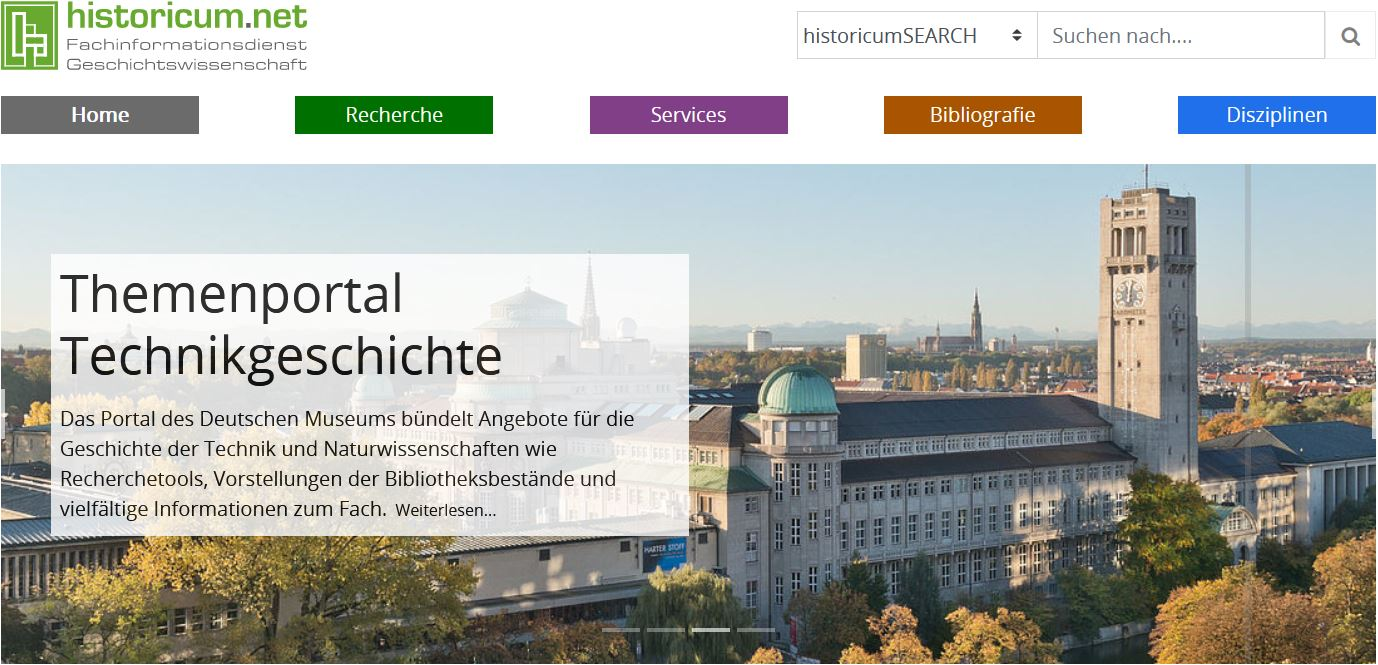
\includegraphics[width=.70\textwidth]{img/Abb7.jpg}
\caption{Neben Digitalisaten bietet die Bibliothek weitere
Dienstleistungen im Fachinformationsdienst Geschichte an.}
\end{figure}

\hypertarget{fazit-und-ausblick}{%
\section{Fazit und Ausblick}\label{fazit-und-ausblick}}

An der Digitalisierungsgeschichte der Bibliothek des Deutschen Museums
werden exemplarisch einige der Grundprobleme deutlich, denen sich jede
Bibliothek stellen muss, die das vermeintlich sichere Terrain einer rein
analogen Literaturversorgung verlassen kann und möchte. Sicherlich liegt
ein Teil der Aufgaben von Bibliotheken weiterhin in der Ermittlung der
passenden (gedruckten und digitalen) Literatur für die jeweiligen
NutzerInnen sowie der Gestaltung und Bereitstellung von attraktiven
Dritten Räumen für die Auseinandersetzung des Einzelnen mit Texten. Der
digitale Wandel und neue Arbeitsformen (sowohl wissenschaftlich als auch
privat) machen bibliothekarische Arbeit aber ebenso notwendig, wie sie
durch Erschließung, Kontextualisierung und Vernetzung Mehrwert
generiert.

Auch weiterhin bleibt es eine Illusion, dass man \enquote{alles im
Internet} finden könne, allein das Urheberrecht setzt hier exakt
bestimmbare Grenzen. Allerdings konnte die Bibliothek einen Teil der
älteren Literatur erfolgreich online bringen. Zur Relation: Die
Public-Private-Partnerschaft mit Google brachte bis heute circa 50.000
Werke ins Netz, der Bestand liegt jedoch bei circa einer Million Bänden
und stellt mittels bibliothekarisch erstellter Metadaten die
Möglichkeiten des Auffindens durch seinen Katalog bereit. Dieser ist
jedoch ebenfalls in andere Portale (Rechercheportale des Verbunds oder
Fachportal des FID) eingebunden. In Ergänzung zu den Anstrengungen in
der Welt der Bücher ist die Bibliothek auch Bestandteil des
Wissenskosmos Deutsches Museum und kommt damit zu ihren Ursprüngen auf
die Münchener Museumsinsel zurück: Im Deutschen Museum
Digital\footnote{\url{https://digital.deutsches-museum.de/} Zugriff am
  08.02.2021.} werden nicht nur ihre (Buch-)Digitalisate, sondern auch
diejenigen der Objektsammlungen und des Archivs gebündelt
werden.\footnote{Huguenin, Fabienne: Deutsches Museum Digital:
  Online-Portal von Archiv, Bibliothek und Objektsammlung. -- In:
  AKMB-news 25 (2019) 2, S. 3--11.}

\hypertarget{literatur}{%
\section{Literatur}\label{literatur}}

\begin{itemize}
\item
  Altenhöner, Reinhard {[}u.a.{]}: Digitalisierung von Kulturgut. In:
   Rolf Griebel {[}u.a.{]} (Hg.): Praxishandbuch
  Bibliotheksmanagement.  Berlin: De Gruyter, 2015, S.
  763--811.
\item
  Bunge, Eva {[}u.a.{]}: Neue Services für die Technikgeschichte:
   Fachinformationsdienst Geschichtswissenschaft (FID). --
  In:  Technikgeschichte 85 (2018), S. 195--201.
\item
  Ceynowa, Klaus: Massendigitalisierung für die Wissenschaft -- Zur
   Digitalisierungsstrategie der Bayerischen
  Staatsbibliothek. In:  Rolf Griebel {[}u.a.{]} (Hg.):
  Information, Innovation, Inspiration.  450 Jahre
  Bayerische Staatsbibliothek. München: Saur, 2008, S. 
  241--252
\item
  Ewert, Gisela {[}u.a.{]}: Bibliotheken. Die Definition der Bibliothek.
   In: Bibliotheksdienst 33 (1999) 6, S. 957--971.
\item
  Fieseler, Christian: Das Verzeichnis Deutscher Drucke des 18.
   Jahrhunderts (VD 18): Ziele, Entwicklung und aktueller
  Stand). --  In BuB 68 (2016) 7, S. 402--405.
\item
  Hilpert, Wilhelm: 10 Jahre Partnerschaft mit Google. Auswirkungen
   und Spuren an der Bayerischen Staatsbibliothek. -- In:
  Klaus  Ceynowa {[}u.a.{]} (Hg.): Bibliotheken:
  Innovation aus Tradition:  Rolf Griebel zum 65.
  Geburtstag. -- Berlin/Boston: De Gruyter,  2015, S.
  258--266.
\item
  Hilz, Helmut (2017): Die Bibliothek des Deutschen Museums.
   Geschichte -- Sammlung -- Bücherschätze. München:
  Deutsches  Museum.
\item
  Huguenin, Fabienne: Deutsches Museum Digital: Online-Portal von
   Archiv, Bibliothek und Objektsammlung. -- In: AKMB-news
  25 (2019)  2, S. 3--11.
\end{itemize}

%autor
\begin{center}\rule{0.5\linewidth}{0.5pt}\end{center}

\textbf{Christian Winkler} hat Romanistik und Geschichtswissenschaft
studiert und ist seit 2018 Mitarbeiter im FID Geschichtswissenschaft und
Leiter des Benutzungsbetriebs und des Google-Projekts der Bibliothek des
Deutschen Museums.

\end{document}
